\section{Overview}

\begin{figure}[b]
	\centering
	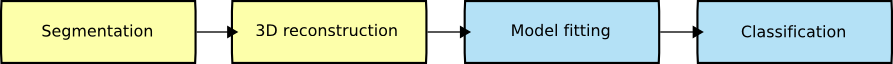
\includegraphics[width=12cm]{overview.png}
	\caption{The main stages in gait recognition.
		Those coloured blue are the ones tackled in this project.}
	\label{OverviewBoxes}
\end{figure}

The continued growth of low-cost high-performance computer hardware has made computer vision increasingly attractive as a means for tackling the problems of biometrics and person indentification.
This project aims to apply computer vision techniques to 3D model fitting with the goal of identifying a person by their gait.

The four main stages in gait recognition are shown in Figure \ref{OverviewBoxes}.
Our data was obtained from the University of Southampton Gait Tunnel -
a walkway in which the walls are lined with a number of cameras to capture images of the subject's face and ears, as well as the motion of his legs and body as he walks.
This data takes the form of several colour videos, so the first step is to isolate the walking figure by segmentation and background subtraction.
Next all these videos are combined together into one three-dimensional video in a process known as 3D reconstruction.

Now we have a single 3D video, the next stage is to extract information that will be able to identify the subject.
We do this by attempting to fit a model to the subject's legs.
This will give us a set of parameters that describe certain properties of the legs in each frame - eg. their angle made with the hip.
By looking at how these parameters change over time, we can form a signature that uniquely describes the subject.
Comparing the signature to a database of other signatures allows us to classify the subject and determine his identity.

This project will only focus on the final two stages - the model fitting and classification.
The data we use for testing has already undergone 3D reconstruction and is in the form of a series of frames containing a voxelized image of the subject.
